\documentclass[10pt]{article}
\usepackage[T1]{fontenc}
\usepackage[utf8]{inputenc}
%\DeclareUnicodeCharacter{00A0}{ }
\usepackage[adobe-utopia]{mathdesign}

\usepackage{amsmath}
\usepackage[francais]{babel}
\usepackage[dvips]{graphicx}
%\usepackage{here}
\usepackage{framed}
\usepackage[normalem]{ulem}
\usepackage{fancyhdr}
\usepackage{titlesec}
\usepackage{vmargin}

\usepackage{amsmath}
\usepackage{ifthen}
\usepackage{multirow}
\usepackage{multicol} % Portions de texte en colonnes

%\usepackage{xltxtra} % Logo XeLaTeX
%\usepackage{pst-solides3d}
\usepackage{color}
%\usepackage{colortbl}
\usepackage{titletoc} % Pour la mise en forme de la table des matières

%\usepackage[crop=off]{auto-pst-pdf}
%\usepackage{bclogo}


%\usepackage{longtable}
%\usepackage{flafter}%floatants après la référence
%\usepackage{pst-solides3d}
%\usepackage{pstricks}
%\usepackage{minitoc}
%\setcounter{minitocdepth}{4}
%\usepackage{draftcopy}% "Brouillon"
%\usepackage{floatflt}
%\usepackage{psfrag}
%\usepackage{listings} % Permet d'insérer du code de programmation
%\usepackage{lmodern}
%\usepackage[adobe-utopia,uppercase=upright,greeklowercase=upright]{mathdesign}
%\usepackage{minionpro}
%\usepackage{pifont}
%\usepackage{amssymb}
%\usepackage[francais]{varioref}

\setmarginsrb{1.5cm}{1cm}{1cm}{1.5cm}{1cm}{1cm}{1cm}{1cm}

\definecolor{gris25}{gray}{0.75}
\definecolor{bleu}{RGB}{18,33,98}
\definecolor{bleuf}{RGB}{42,94,171}
\definecolor{bleuc}{RGB}{231,239,247}
\definecolor{rougef}{RGB}{185,18,27}
\definecolor{rougec}{RGB}{255,230,231}
\definecolor{vertf}{RGB}{103,126,82}
\definecolor{vertc}{RGB}{220,255,191}
\definecolor{violetf}{RGB}{112,48,160}
\definecolor{violetc}{RGB}{230,224,236}
\definecolor{jaunec}{RGB}{220,255,191}
%\usepackage{algorithm}
%\usepackage{algorithmic}
\usepackage[french]{algorithm2e}

\SetKwBlock{Fonction}{Début Fonction}{Fin Fonction}
\SetKwComment{Comment}{start}{end}
% Python sources

\usepackage{listings}
\lstloadlanguages{R}   % pour regler les pb d accent utf8 dans les codes
\lstset{language=R} % pour regler les pb d accent utf8 dans les codes

\usepackage{textcomp}
\usepackage{setspace}
%\usepackage{palatino}

%\usepackage{color}
\definecolor{Bleu}{rgb}{0.1,0.1,1.0}
\definecolor{Noir}{rgb}{0,0,0}
\definecolor{Grau}{rgb}{0.5,0.5,0.5}
\definecolor{DunkelGrau}{rgb}{0.15,0.15,0.15}
\definecolor{Hellbraun}{rgb}{0.5,0.25,0.0}
\definecolor{Magenta}{rgb}{1.0,0.0,1.0}
\definecolor{Gris}{gray}{0.5}
\definecolor{Vert}{rgb}{0,0.5,0}
\definecolor{SourceHintergrund}{rgb}{1,1.0,0.95}


%
\renewcommand{\lstlistlistingname}{Listings}
\renewcommand{\lstlistingname}{Listing}

\lstnewenvironment{python}[1][]{
\lstset{
%escapeinside={\%*}{*)},
%inputencoding=utf8,   % pour regler les pb d accent utf8 dans les codes
%extendedchars=true,   % pour regler les pb d accent utf8 dans les codes
language=python,
basicstyle=\sffamily\footnotesize, 	
stringstyle=\color{red}, 
showstringspaces=false, 
alsoletter={1234567890},
otherkeywords={\ , \}, \{},
keywordstyle=\color{blue},
emph={access,and,break,class,continue,def,del,elif ,else,
except,exec,finally,for,from,global,if,import,in,i s,
lambda,not,or,pass,print,raise,return,try,while},
emphstyle=\color{black}\bfseries,
emph={[2]True, False, None, self},
emphstyle=[2]\color{black},
emph={[3]from, import, as},
emphstyle=[3]\color{blue},
upquote=true,
columns=flexible, % pour empecher d'avoir un espacement mono
morecomment=[s]{"""}{"""},
commentstyle=\color{Hellbraun}\slshape, 
%emph={[4]1, 2, 3, 4, 5, 6, 7, 8, 9, 0},
emphstyle=[4]\color{blue},
literate=*{:}{{\textcolor{blue}:}}{1}
{=}{{\textcolor{blue}=}}{1}
{-}{{\textcolor{blue}-}}{1}
{+}{{\textcolor{blue}+}}{1}
{*}{{\textcolor{blue}*}}{1}
{!}{{\textcolor{blue}!}}{1}
{(}{{\textcolor{blue}(}}{1}
{)}{{\textcolor{blue})}}{1}
{[}{{\textcolor{blue}[}}{1}
{]}{{\textcolor{blue}]}}{1}
{<}{{\textcolor{blue}<}}{1}
{>}{{\textcolor{blue}>}}{1}
{COMPLETER}{{\textcolor{red}COMPLETER}}{1},
literate=%
            {é}{{\'{e}}}1
            {è}{{\`{e}}}1
            {ê}{{\^{e}}}1
            {ë}{{\¨{e}}}1
            {û}{{\^{u}}}1
            {ù}{{\`{u}}}1
            {â}{{\^{a}}}1
            {à}{{\`{a}}}1
            {î}{{\^{i}}}1
            {ç}{{\c{c}}}1
            {Ç}{{\c{C}}}1
            {É}{{\'{E}}}1
            {Ê}{{\^{E}}}1
            {À}{{\`{A}}}1
            {Â}{{\^{A}}}1
            {Î}{{\^{I}}}1, % pour regler les pb d accent utf8 dans les codes
            numbers=right, % where to put the line-numbers; possible values are (none, left, right)
           numbersep=-10pt,
%framexleftmargin=1mm, framextopmargin=1mm, frame=shadowbox, rulesepcolor=\color{blue},#1
%backgroundcolor=\color{SourceHintergrund}, 
%framexleftmargin=1mm, framexrightmargin=1mm, framextopmargin=1mm, frame=single, framerule=1pt, rulecolor=\color{black},#1
}}{}



\lstnewenvironment{scilab}[1][]{
\lstset{
language=scilab,
basicstyle=\sffamily\footnotesize, 	
stringstyle=\color{red}, 
showstringspaces=false, 
alsoletter={1234567890},
otherkeywords={\ , \}, \{},
keywordstyle=\color{blue},
emph={access,and,break,class,continue,def,del,elif ,else,
except,exec,finally,for,from,global,if,import,in,i s,
lambda,not,or,pass,print,raise,return,try,while,Debut},
emphstyle=\color{black}\bfseries,
emph={[2]True, False, None, self},
emphstyle=[2]\color{olive},
emph={[3]from, import, as},
emphstyle=[3]\color{blue},
upquote=true,
columns=flexible, % pour empecher d'avoir un espacement mono
morecomment=[s]{"""}{"""},
commentstyle=\color{Hellbraun}\slshape, 
%emph={[4]1, 2, 3, 4, 5, 6, 7, 8, 9, 0},
emphstyle=[4]\color{blue},
literate=*{:}{{\textcolor{blue}:}}{1}
{=}{{\textcolor{blue}=}}{1}
{-}{{\textcolor{blue}-}}{1}
{+}{{\textcolor{blue}+}}{1}
{*}{{\textcolor{blue}*}}{1}
{!}{{\textcolor{blue}!}}{1}
{(}{{\textcolor{blue}(}}{1}
{)}{{\textcolor{blue})}}{1}
{[}{{\textcolor{blue}[}}{1}
{]}{{\textcolor{blue}]}}{1}
{<}{{\textcolor{blue}<}}{1}
{>}{{\textcolor{blue}>}}{1},
%framexleftmargin=1mm, framextopmargin=1mm, frame=shadowbox, rulesepcolor=\color{blue},#1
%backgroundcolor=\color{SourceHintergrund}, 
%framexleftmargin=1mm, framexrightmargin=1mm, framextopmargin=1mm, frame=single, framerule=1pt, rulecolor=\color{black},#1
}}{}


\lstdefinestyle{stylepython}{%
escapeinside={\%*}{*)},
inputencoding=utf8,   % pour regler les pb d accent utf8 dans les codes
extendedchars=true,   % pour regler les pb d accent utf8 dans les codes
language=python,
basicstyle=\sffamily\footnotesize, 	
stringstyle=\color{red}, 
showstringspaces=false, 
alsoletter={1234567890},
otherkeywords={\ , \}, \{},
keywordstyle=\color{blue},
emph={access,and,break,class,continue,def,del,elif ,else,
except,exec,finally,for,from,global,if,import,in,i s,
lambda,not,or,pass,print,raise,return,try,while},
emphstyle=\color{black}\bfseries,
emph={[2]True, False, None, self},
emphstyle=[2]\color{green},
emph={[3]from, import, as},
emphstyle=[3]\color{blue},
upquote=true,
columns=flexible, % pour empecher d'avoir un espacement mono
morecomment=[s]{"""}{"""},
commentstyle=\color{Hellbraun}\slshape, 
%emph={[4]1, 2, 3, 4, 5, 6, 7, 8, 9, 0},
emphstyle=[4]\color{blue},
literate=*{:}{{\textcolor{blue}:}}{1}
{=}{{\textcolor{blue}=}}{1}
{-}{{\textcolor{blue}-}}{1}
{+}{{\textcolor{blue}+}}{1}
{*}{{\textcolor{blue}*}}{1}
{!}{{\textcolor{blue}!}}{1}
{(}{{\textcolor{blue}(}}{1}
{)}{{\textcolor{blue})}}{1}
{[}{{\textcolor{blue}[}}{1}
{]}{{\textcolor{blue}]}}{1}
{<}{{\textcolor{blue}<}}{1}
{>}{{\textcolor{blue}>}}{1}
{COMPLETER}{{\textcolor{red}COMPLETER}}{1},
literate=%
            {é}{{\'{e}}}1
            {è}{{\`{e}}}1
            {ê}{{\^{e}}}1
            {ë}{{\¨{e}}}1
            {û}{{\^{u}}}1
            {ù}{{\`{u}}}1
            {â}{{\^{a}}}1
            {à}{{\`{a}}}1
            {î}{{\^{i}}}1
            {ç}{{\c{c}}}1
            {Ç}{{\c{C}}}1
            {É}{{\'{E}}}1
            {Ê}{{\^{E}}}1
            {À}{{\`{A}}}1
            {Â}{{\^{A}}}1
            {Î}{{\^{I}}}1,
%numbers=left,                    % where to put the line-numbers; possible values are (none, left, right)
%numbersep=5pt,                   % how far the line-numbers are from the code
%numberstyle=\tiny\color{mygray}, % the style that is used for the line-numbers
}

%
%\renewcommand{\algorithmicrequire} {\textbf{\textsc{Entrées:}}}
%\renewcommand{\algorithmicensure}  {\textbf{\textsc{Sorties:}}}
%\renewcommand{\algorithmicwhile}   {\textbf{tantque}}
%\renewcommand{\algorithmicdo}      {\textbf{faire}}
%\renewcommand{\algorithmicendwhile}{\textbf{fin tantque}}
%\renewcommand{\algorithmicend}     {\textbf{fin}}
%\renewcommand{\algorithmicif}      {\textbf{si}}
%\renewcommand{\algorithmicendif}   {\textbf{finsi}}
%\renewcommand{\algorithmicelse}    {\textbf{sinon}}
%\renewcommand{\algorithmicthen}    {\textbf{alors}}
%\renewcommand{\algorithmicfor}     {\textbf{pour}}
%\renewcommand{\algorithmicforall}  {\textbf{pour tout}}
%\renewcommand{\algorithmicdo}      {\textbf{faire}}
%\renewcommand{\algorithmicendfor}  {\textbf{fin pour}}
%\renewcommand{\algorithmicloop}    {\textbf{boucler}}
%\renewcommand{\algorithmicendloop} {\textbf{fin boucle}}
%\renewcommand{\algorithmicrepeat}  {\textbf{répéter}}
%\renewcommand{\algorithmicuntil}   {\textbf{jusqu'à}}

\lstnewenvironment{termi}[1][]{
\lstset{
language=scilab,
basicstyle=\sffamily\footnotesize, 	
stringstyle=\color{red}, 
showstringspaces=false, 
alsoletter={1234567890},
otherkeywords={\ , \}, \{},
keywordstyle=\color{blue},
emph={access,and,break,class,continue,def,del,elif ,else,
except,exec,finally,for,from,global,if,import,in,i s,
lambda,not,or,pass,print,raise,return,try,while,Debut},
emphstyle=\color{black}\bfseries,
emph={[2]True, False, None, self},
emphstyle=[2]\color{green},
emph={[3]from, import, as},
emphstyle=[3]\color{blue},
upquote=true,
columns=flexible, % pour empecher d'avoir un espacement mono
morecomment=[s]{"""}{"""},
commentstyle=\color{Hellbraun}\slshape, 
%emph={[4]1, 2, 3, 4, 5, 6, 7, 8, 9, 0},
emphstyle=[4]\color{blue},
literate=*{:}{{\textcolor{blue}:}}{1}
{=}{{\textcolor{blue}=}}{1}
{-}{{\textcolor{blue}-}}{1}
{+}{{\textcolor{blue}+}}{1}
{*}{{\textcolor{blue}*}}{1}
{!}{{\textcolor{blue}!}}{1}
{(}{{\textcolor{blue}(}}{1}
{)}{{\textcolor{blue})}}{1}
{[}{{\textcolor{blue}[}}{1}
{]}{{\textcolor{blue}]}}{1}
{<}{{\textcolor{blue}<}}{1}
{>}{{\textcolor{blue}>}}{1},
%framexleftmargin=1mm, framextopmargin=1mm, frame=shadowbox, rulesepcolor=\color{blue},#1
%backgroundcolor=\color{SourceHintergrund}, 
%framexleftmargin=1mm, framexrightmargin=1mm, framextopmargin=1mm, frame=single, framerule=1pt, rulecolor=\color{black},#1
}}{}


\lstnewenvironment{sql}[1][]{
\lstset{
%escapeinside={\%*}{*)},
%inputencoding=utf8,   % pour regler les pb d accent utf8 dans les codes
%extendedchars=true,   % pour regler les pb d accent utf8 dans les codes
language=sql,
basicstyle=\sffamily\footnotesize, 	
stringstyle=\color{red}, 
showstringspaces=false, 
alsoletter={1234567890},
otherkeywords={\ , \}, \{},
keywordstyle=\color{blue},
emph={access,and,break,class,continue,def,del,elif ,else,
except,exec,finally,for,from,global,if,import,in,i s,
lambda,not,or,pass,print,raise,return,try,while},
emphstyle=\color{black}\bfseries,
emph={[2]True, False, None, self},
emphstyle=[2]\color{olive},
emph={[3]from, import, as},
emphstyle=[3]\color{blue},
upquote=true,
columns=flexible, % pour empecher d'avoir un espacement mono
morecomment=[s]{"""}{"""},
commentstyle=\color{Hellbraun}\slshape, 
%emph={[4]1, 2, 3, 4, 5, 6, 7, 8, 9, 0},
emphstyle=[4]\color{blue},
literate=*{:}{{\textcolor{blue}:}}{1}
{=}{{\textcolor{blue}=}}{1}
{-}{{\textcolor{blue}-}}{1}
{+}{{\textcolor{blue}+}}{1}
{*}{{\textcolor{blue}*}}{1}
{!}{{\textcolor{blue}!}}{1}
{(}{{\textcolor{blue}(}}{1}
{)}{{\textcolor{blue})}}{1}
{[}{{\textcolor{blue}[}}{1}
{]}{{\textcolor{blue}]}}{1}
{<}{{\textcolor{blue}<}}{1}
{>}{{\textcolor{blue}>}}{1}
{COMPLETER}{{\textcolor{red}COMPLETER}}{1},
literate=%
            {é}{{\'{e}}}1
            {è}{{\`{e}}}1
            {ê}{{\^{e}}}1
            {ë}{{\¨{e}}}1
            {û}{{\^{u}}}1
            {ù}{{\`{u}}}1
            {â}{{\^{a}}}1
            {à}{{\`{a}}}1
            {î}{{\^{i}}}1
            {ç}{{\c{c}}}1
            {Ç}{{\c{C}}}1
            {É}{{\'{E}}}1
            {Ê}{{\^{E}}}1
            {À}{{\`{A}}}1
            {Â}{{\^{A}}}1
            {Î}{{\^{I}}}1, % pour regler les pb d accent utf8 dans les codes
%framexleftmargin=1mm, framextopmargin=1mm, frame=shadowbox, rulesepcolor=\color{blue},#1
%backgroundcolor=\color{SourceHintergrund}, 
%framexleftmargin=1mm, framexrightmargin=1mm, framextopmargin=1mm, frame=single, framerule=1pt, rulecolor=\color{black},#1
}}{}


%
%\renewcommand{\algorithmicrequire} {\textbf{\textsc{Entrées:}}}
%\renewcommand{\algorithmicensure}  {\textbf{\textsc{Sorties:}}}
%\renewcommand{\algorithmicwhile}   {\textbf{tantque}}
%\renewcommand{\algorithmicdo}      {\textbf{faire}}
%\renewcommand{\algorithmicendwhile}{\textbf{fin tantque}}
%\renewcommand{\algorithmicend}     {\textbf{fin}}
%\renewcommand{\algorithmicif}      {\textbf{si}}
%\renewcommand{\algorithmicendif}   {\textbf{finsi}}
%\renewcommand{\algorithmicelse}    {\textbf{sinon}}
%\renewcommand{\algorithmicthen}    {\textbf{alors}}
%\renewcommand{\algorithmicfor}     {\textbf{pour}}
%\renewcommand{\algorithmicforall}  {\textbf{pour tout}}
%\renewcommand{\algorithmicdo}      {\textbf{faire}}
%\renewcommand{\algorithmicendfor}  {\textbf{fin pour}}
%\renewcommand{\algorithmicloop}    {\textbf{boucler}}
%\renewcommand{\algorithmicendloop} {\textbf{fin boucle}}
%\renewcommand{\algorithmicrepeat}  {\textbf{répéter}}
%\renewcommand{\algorithmicuntil}   {\textbf{jusqu'à}}
%%%%%%%%%%%%
% Définition des vecteurs 
%%%%%%%%%%%%
 \newcommand{\vect}[1]{\overrightarrow{#1}}
\newcommand{\axe}[2]{\left(#1,\vect{#2}\right)}

\newcommand{\rep}[1]{\mathcal{R}_{#1}}
\newcommand{\vx}[1]{\vect{x_{#1}}}
\newcommand{\vy}[1]{\vect{y_{#1}}}
\newcommand{\vz}[1]{\vect{z_{#1}}}

%%%%%%%%%%%%
% Définition des torseurs 
%%%%%%%%%%%%

 \newcommand{\torseur}[1]{%
\left\{{#1}\right\}
}

\newcommand{\torseurcin}[3]{%
\left\{\mathcal{#1} \left(#2/#3 \right) \right\}
}

\newcommand{\torseurstat}[3]{%
\left\{\mathcal{#1} \left(#2\rightarrow #3 \right) \right\}
}

 \newcommand{\torseurc}[8]{%
%\left\{#1 \right\}=
\left\{
{#1}
\right\}
 = 
\left\{%
\begin{array}{cc}%
{#2} & {#5}\\%
{#3} & {#6}\\%
{#4} & {#7}\\%
\end{array}%
\right\}_{#8}%
}

 \newcommand{\torseurcol}[7]{
\left\{%
\begin{array}{cc}%
{#1} & {#4}\\%
{#2} & {#5}\\%
{#3} & {#6}\\%
\end{array}%
\right\}_{#7}%
}

 \newcommand{\torseurl}[3]{%
%\left\{\mathcal{#1}\right\}_{#2}=%
\left\{%
\begin{array}{l}%
{#1} \\%
{#2} %
\end{array}%
\right\}_{#3}%
}

 \newcommand{\vectv}[3]{%
\vect{V\left( {#1} \in {#2}/{#3}\right)}
}


\newcommand{\vectf}[2]{%
\vect{R\left( {#1} \rightarrow {#2}\right)}
}

\newcommand{\vectm}[3]{%
\vect{\mathcal{M}\left( {#1}, {#2} \rightarrow {#3}\right)}
}


 \newcommand{\vectg}[3]{%
\vect{\Gamma \left( {#1} \in {#2}/{#3}\right)}
}

 \newcommand{\vecto}[2]{%
\vect{\Omega\left( {#1}/{#2}\right)}
}
% }$$\left\{\mathcal{#1} \right\}_{#2} =%
% \left\{%
% \begin{array}{c}%
%  #3 \\%
%  #4 %
% \end{array}%
% \right\}_{#5}}
\setcounter{tocdepth}{2}
% \mtcselectlanguage{french} 


%  ------------------------------------------
% | Modification du formatage des sections : | 
%  ------------------------------------------

% Grands titres :
% ---------------

\newcommand{\titre}[1]{%
\begin{center}
      \bigskip
      \rule{\textwidth}{1pt}
      \par\vspace{0.1cm}
      
      \textbf{\large #1}
      \par\rule{\textwidth}{1pt}
    \end{center}
    \bigskip
  }

% Supprime le numéro du chapitre dans la numérotation des sections:
% -----------------------------------------------------------------
\makeatletter
\renewcommand{\thesection}{\@arabic\c@section}
\makeatother


% \titleformat{\chapter}[display]
% {\normalfont\Large\filcenter}
% {}
% {1pc}
% {\titlerule[1pt]
%   \vspace{1pc}%
%   \Huge}[\vspace{1ex}%
% \titlerule]


%%%% Chapitres Comme PY Pechard %%%%%%%%%
% numéro du chapitre
\DeclareFixedFont{\chapnumfont}{OT1}{phv}{b}{n}{80pt}
% pour le mot « Chapitre »
\DeclareFixedFont{\chapchapfont}{OT1}{phv}{m}{it}{40pt}
% pour le titre
\DeclareFixedFont{\chaptitfont}{T1}{phv}{b}{n}{25pt}

\definecolor{gris}{gray}{0.75}
\titleformat{\chapter}[display]%
	{\sffamily}%
	{\filleft\chapchapfont\color{gris}\chaptertitlename\
	\\
	\vspace{12pt}
	\chapnumfont\thechapter}%
	{16pt}%
	{\filleft\chaptitfont}%
	[\vspace{6pt}\titlerule\titlerule\titlerule]

%%%%  Fin Chapitres Comme PY Pechard %%%%%%%%%


% Section, subsection, subsubsection sans serifs :
% % ----------------------------------------------

% \makeatletter
% \renewcommand{\section}{\@startsection{section}{0}{0mm}%
% {\baselineskip}{.3\baselineskip}%
% {\normalfont\sffamily\Large\textbf}}%
% \makeatother

\makeatletter
\renewcommand{\@seccntformat}[1]{{\textcolor{bleu}{\csname
the#1\endcsname}\hspace{0.5em}}}
\makeatother

\makeatletter
\renewcommand{\section}{\@startsection{section}{1}{\z@}%
                       {-4ex \@plus -1ex \@minus -.4ex}%
                       {1ex \@plus.2ex }%
                       {\normalfont\Large\sffamily\bfseries}}%
\makeatother
 
\makeatletter
\renewcommand{\subsection}{\@startsection {subsection}{2}{\z@}
                          {-3ex \@plus -0.1ex \@minus -.4ex}%
                          {0.5ex \@plus.2ex }%
                          {\normalfont\large\sffamily\bfseries}}
\makeatother
 
\makeatletter
\renewcommand{\subsubsection}{\@startsection {subsubsection}{3}{\z@}
                          {-2ex \@plus -0.1ex \@minus -.2ex}%
                          {0.2ex \@plus.2ex }%
                          {\normalfont\large\sffamily\bfseries}}
\makeatother
 
\makeatletter             
\renewcommand{\paragraph}{\@startsection{paragraph}{4}{\z@}%
                                    {-2ex \@plus-.2ex \@minus .2ex}%
                                    {0.1ex}%               
{\normalfont\sffamily\bfseries}}
\makeatother
 
 
\makeatletter             
\renewcommand{\subparagraph}{\@startsection{subparagraph}{5}{\z@}%
                                    {-2ex \@plus-.2ex \@minus .2ex}%
                                    {0ex}%               
{\normalfont\bfseries Question }}
\makeatother
\renewcommand{\thesubparagraph}{\arabic{subparagraph}} 
\makeatletter

\setcounter{secnumdepth}{5}





% Formatage de la table des matières 
% Paquets nécessaires : titletoc ?

% Chapitre spéciaux écrits dans un nombre cerclé dans la table des matières.
\titlecontents{chapter}[+3pc]
  {\addvspace{10pt}\sffamily\bfseries}
{\contentslabel[{\pscirclebox[fillstyle=solid,fillcolor=gray!25,
linecolor=gray!25,framesep=4pt]{\textcolor{white}{\thecontentslabel}}}]{2.5pc}}
  {}
  {\dotfill \normalfont\thecontentspage\ }

\titlecontents{section}[3pc]
  {\addvspace{2pt}\sffamily}
  {\contentslabel[\thecontentslabel]{1.8pc}}
  {}
  {\dotfill \normalfont\thecontentspage\ }

\titlecontents{subsection}[5pc]
  {\addvspace{2pt}\sffamily}
  {\contentslabel[\thecontentslabel]{1.8pc}}
  {}
  {\dotfill \normalfont\thecontentspage\ }

\titlecontents{subsubsection}[8pc]
  {\addvspace{2pt}\sffamily}
  {\contentslabel[\thecontentslabel]{3pc}}
  {}
  {\dotfill \normalfont\thecontentspage\ }
%{\;\titlerule\;\normalfont\thecontentspage\ }

\titlecontents{paragraph}[9pc]
  {\addvspace{2pt}\sffamily}
  {\contentslabel[\thecontentslabel]{3.5pc}}
  {}
  {\dotfill \normalfont\thecontentspage\ }

%pour avoir l indentation dans minipage
\newdimen\oldparindent\oldparindent=\parindent

\makeatletter
\def\@iiiminipage#1#2[#3]#4{%
  \noindent
  \leavevmode
  \@pboxswfalse
  \setlength\@tempdima{#4}%
  \def\@mpargs{{#1}{#2}[#3]{#4}}%
  \setbox\@tempboxa\vbox\bgroup
    \color@begingroup
      \hsize\@tempdima
      \textwidth\hsize \columnwidth\hsize
      \@parboxrestore
      \parindent=\oldparindent
      \def\@mpfn{mpfootnote}\def\thempfn{\thempfootnote}\c@mpfootnote\z@
      \let\@footnotetext\@mpfootnotetext
      \let\@listdepth\@mplistdepth \@mplistdepth\z@
      \@minipagerestore
      \@setminipage}
\makeatother

% Paquets requis : 

\definecolor{gris25}{gray}{0.75}
\definecolor{bleu}{RGB}{18,33,98}
\definecolor{bleuf}{RGB}{42,94,171}
\definecolor{bleuc}{RGB}{231,239,247}
\definecolor{rougef}{RGB}{185,18,27}
\definecolor{rougec}{RGB}{255,230,231}
\definecolor{vertf}{RGB}{103,126,82}
\definecolor{vertc}{RGB}{220,255,191}
\definecolor{violetf}{RGB}{112,48,160}
\definecolor{violetc}{RGB}{230,224,236}
\definecolor{jaunec}{RGB}{220,255,191}



\newenvironment{corrige}[1][\hsize]%
{%
    \def\FrameCommand%
    {%
\rotatebox{90}{\textit{\textsf{Corrigé}}} 
        {\color{violetf}\vrule width 3pt}%
        \hspace{0pt}%must no space.
        \fboxsep=\FrameSep\colorbox{violetc}%
    }%
    \MakeFramed{\hsize #1 \advance\hsize-\width\FrameRestore}%
}%
{\endMakeFramed}%

\newenvironment{sci}[1][\hsize]%
{%
    \def\FrameCommand%
    {%
%\rotatebox{90}{\textit{\textsf{Scilab}}
\includegraphics[height=.8cm]{png/logo_scilab}} 
\rotatebox{90}{
\includegraphics[height=.6cm]{png/logo_scilab}} 
        {\color{violetf}\vrule width 3pt}%
        \hspace{0pt}%must no space.
        \fboxsep=\FrameSep\colorbox{violetc}%
    }%
    \MakeFramed{\hsize #1 \advance\hsize-\width\FrameRestore}%
}%
{\endMakeFramed}%

\newenvironment{pseudo}[1][\hsize]%
{%
    \def\FrameCommand%
    {%
\rotatebox{90}{\textit{\textsf{Pseudo Code}}} 
        {\color{violetf}\vrule width 3pt}%
        \hspace{0pt}%must no space.
        \fboxsep=\FrameSep\colorbox{violetc}%
    }%
    \MakeFramed{\hsize #1 \advance\hsize-\width\FrameRestore}%
}%
{\endMakeFramed}%

\newenvironment{py}[1][\hsize]%
{%
    \def\FrameCommand%
    {%
%\rotatebox{90}{\textit{\textsf{Python}}} 
\rotatebox{90}{
\includegraphics[height=.6cm]{png/logo_python}} 
        {\color{violetf}\vrule width 3pt}%
        \hspace{0pt}%must no space.
        \fboxsep=\FrameSep\colorbox{violetc}%
    }%
    \MakeFramed{\hsize #1 \advance\hsize-\width\FrameRestore}%
}%
{\endMakeFramed}%


\newenvironment{term}[1][\hsize]%
{%
    \def\FrameCommand%
    {%
\rotatebox{90}{\textit{\textsf{Terminal}}} 
        {\color{violetf}\vrule width 3pt}%
        \hspace{0pt}%must no space.
        \fboxsep=\FrameSep\colorbox{violetc}%
    }%
    \MakeFramed{\hsize #1 \advance\hsize-\width\FrameRestore}%
}%
{\endMakeFramed}%



\newenvironment{comp}[1][\hsize]%
{%
    \def\FrameCommand
    {%
\rotatebox{90}{\textit{\textsf{Compétences}}} 
        {\color{bleuf}\vrule width 3pt}%
        \hspace{0pt}%must no space.
        \fboxsep=\FrameSep\colorbox{bleuc}%
    }%
    \MakeFramed{\hsize#1\advance\hsize-\width\FrameRestore}%
}%
{\endMakeFramed}%

\newenvironment{rem}[1][\hsize]%
{%
    \def\FrameCommand
    {%
\rotatebox{90}{\textit{\textsf{Remarque}}} 
        {\color{bleuf}\vrule width 3pt}%
        \hspace{0pt}%must no space.
        \fboxsep=\FrameSep\colorbox{bleuc}%
    }%
    \MakeFramed{\hsize#1\advance\hsize-\width\FrameRestore}%
}%
{\endMakeFramed}%


\newenvironment{savoir}[1][\hsize]%
{%
    \def\FrameCommand
    {%
\rotatebox{90}{\textit{\textsf{Savoir}}} 
        {\color{bleuf}\vrule width 3pt}%
        \hspace{0pt}%must no space.
        \fboxsep=\FrameSep\colorbox{bleuc}%
    }%
    \MakeFramed{\hsize#1\advance\hsize-\width\FrameRestore}%
}%
{\endMakeFramed}%

\newenvironment{Objectif}[1][\hsize]%
{%
    \def\FrameCommand
    {%
\rotatebox{90}{\textit{\textsf{Objectif}}} 
        {\color{bleuf}\vrule width 3pt}%
        \hspace{0pt}%must no space.
        \fboxsep=\FrameSep\colorbox{bleuc}%
    }%
    \MakeFramed{\hsize#1\advance\hsize-\width\FrameRestore}%
}%
{\endMakeFramed}%

\newenvironment{prob}[1][\hsize]%
{%
    \def\FrameCommand%
    {%
\rotatebox{90}{\textit{\textsf{ Problématique}}} 
        {\color{rougef}\vrule width 3pt}%
        \hspace{0pt}%must no space.
        \fboxsep=\FrameSep\colorbox{rougec}%
    }%
    \MakeFramed{\hsize#1\advance\hsize-\width\FrameRestore}%
}%
{\endMakeFramed}%

\newenvironment{obj}[1][\hsize]%
{%
    \def\FrameCommand%
    {%
\rotatebox{90}{\textit{\textsf{Objectifs}}} 
        {\color{rougef}\vrule width 3pt}%
        \hspace{0pt}%must no space.
        \fboxsep=\FrameSep\colorbox{rougec}%
    }%
    \MakeFramed{\hsize#1\advance\hsize-\width\FrameRestore}%
}%
{\endMakeFramed}%

\newenvironment{defi}[1][\hsize]%
{%
    \def\FrameCommand%
    {%
\rotatebox{90}{\textit{\textsf{Définition\\}}} 
        {\color{bleuf}\vrule width 3pt}%
        \hspace{0pt}%must no space.
        \fboxsep=\FrameSep\colorbox{bleuc}%
    }%
    \MakeFramed{\hsize#1\advance\hsize-\width\FrameRestore}%
}%
{\endMakeFramed}%


\newenvironment{demo}[1][\hsize]%
{%
    \def\FrameCommand%
    {%
\rotatebox{90}{\textit{\textsf{Démonstration\\}}} 
        {\color{bleuf}\vrule width 3pt}%
        \hspace{0pt}%must no space.
        \fboxsep=\FrameSep\colorbox{bleuc}%
    }%
    \MakeFramed{\hsize#1\advance\hsize-\width\FrameRestore}%
}%
{\endMakeFramed}%


\newenvironment{hypo}[1][\hsize]%
{%
    \def\FrameCommand%
    {%
\rotatebox{90}{\textit{\textsf{Hypothèse\\}}} 
        {\color{bleuf}\vrule width 3pt}%
        \hspace{0pt}%must no space.
        \fboxsep=\FrameSep\colorbox{bleuc}%
    }%
    \MakeFramed{\hsize#1\advance\hsize-\width\FrameRestore}%
}%
{\endMakeFramed}%


\newenvironment{prop}[1][\hsize]%
{%
    \def\FrameCommand%
    {%
\rotatebox{90}{\textit{\textsf{Propriété\\}}} 
        {\color{bleuf}\vrule width 3pt}%
        \hspace{0pt}%must no space.
        \fboxsep=\FrameSep\colorbox{bleuc}%
    }%
    \MakeFramed{\hsize#1\advance\hsize-\width\FrameRestore}%
}%
{\endMakeFramed}%

\newenvironment{props}[1][\hsize]%
{%
    \def\FrameCommand%
    {%
\rotatebox{90}{\textit{\textsf{Propriétés\\}}} 
        {\color{bleuf}\vrule width 3pt}%
        \hspace{0pt}%must no space.
        \fboxsep=\FrameSep\colorbox{bleuc}%
    }%
    \MakeFramed{\hsize#1\advance\hsize-\width\FrameRestore}%
}%
{\endMakeFramed}%

\newenvironment{exemple}[1][\hsize]%
{%
    \def\FrameCommand%
    {%
\rotatebox{90}{\textit{\textsf{Exemple\\}}} 
        {\color{vertf}\vrule width 3pt}%
        \hspace{0pt}%must no space.
        \fboxsep=\FrameSep\colorbox{vertc}%
    }%
    \MakeFramed{\hsize#1\advance\hsize-\width\FrameRestore}%
}%
{\endMakeFramed}%

\newenvironment{exercice}[1][\hsize]%
{%
    \def\FrameCommand%
    {%
\rotatebox{90}{\textit{\textsf{Exercice\\}}} 
        {\color{vertf}\vrule width 3pt}%
        \hspace{0pt}%must no space.
        \fboxsep=\FrameSep\colorbox{vertc}%
    }%
    \MakeFramed{\hsize#1\advance\hsize-\width\FrameRestore}%
}%
{\endMakeFramed}%

\newenvironment{Support}[1][\hsize]%
{%
    \def\FrameCommand%
    {%
\rotatebox{90}{\textit{\textsf{Support de cours\\}}} 
        {\color{vertf}\vrule width 3pt}%
        \hspace{0pt}%must no space.
        \fboxsep=\FrameSep\colorbox{jaunec}%
    }%
    \MakeFramed{\hsize#1\advance\hsize-\width\FrameRestore}%
}%
{\endMakeFramed}%

\newenvironment{resultat}[1][\hsize]%
{%
    \def\FrameCommand%
    {%
\rotatebox{90}{\textit{\textsf{Résultat\\}}} 
        {\color{rougef}\vrule width 3pt}%
        \hspace{0pt}%must no space.
        \fboxsep=\FrameSep\colorbox{rougec}%
    }%
    \MakeFramed{\hsize#1\advance\hsize-\width\FrameRestore}%
}%
{\endMakeFramed}%

\newenvironment{methode}[1][\hsize]%
{%
    \def\FrameCommand%
    {%
\rotatebox{90}{\textit{\textsf{Méthode\\}}} 
        {\color{rougef}\vrule width 3pt}%
        \hspace{0pt}%must no space.
        \fboxsep=\FrameSep\colorbox{rougec}%
    }%
    \MakeFramed{\hsize#1\advance\hsize-\width\FrameRestore}%
}%
{\endMakeFramed}%

\newenvironment{theo}[1][\hsize]%
{%
    \def\FrameCommand%
    {%
\rotatebox{90}{\textit{\textsf{Théorème\\}}} 
        {\color{rougef}\vrule width 3pt}%
        \hspace{0pt}%must no space.
        \fboxsep=\FrameSep\colorbox{rougec}%
    }%
    \MakeFramed{\hsize#1\advance\hsize-\width\FrameRestore}%
}%
{\endMakeFramed}%

\newenvironment{warn}[1][\hsize]%
{%
    \def\FrameCommand%
    {%
\rotatebox{90}{\textit{\textsf{Attention\\}}} 
        {\color{rougef}\vrule width 3pt}%
        \hspace{0pt}%must no space.
        \fboxsep=\FrameSep\colorbox{rougec}%
    }%
    \MakeFramed{\hsize#1\advance\hsize-\width\FrameRestore}%
}%
{\endMakeFramed}%


%Si le boolen xp est vrai : compilation pour xabi
%Sinon compilation Damien
\newboolean{xp}
\setboolean{xp}{true}

\newboolean{prof}
\setboolean{prof}{false}

\def\xxtitre{\ifthenelse{\boolean{xp}}{
CI 3 : Ingénierie Numérique \& Simulation
}}

\def\xxsoustitre{\ifthenelse{\boolean{xp}}{
TP -- Résolution d'équations différentielles}{
}}


\def\xxauteur{\ifthenelse{\boolean{xp}}{
\noindent \textsl{Cédric Lopez} \\
\textsl{Xavier Pessoles}
}{
}}


\def\xxpied{\ifthenelse{\boolean{xp}}{
CI 3 : Ingénierie Numérique \& Simulation -- TP \\
Résolution d'équations différentielles -- \ifthenelse{\boolean{prof}}{P}{E}%
}{
}}

\usepackage[%
    pdftitle={Ingénierie Numérique et Simulation},
    pdfauthor={Xavier Pessoles},
    colorlinks=true,
    linkcolor=blue,
    citecolor=magenta]{hyperref}



\usepackage{pifont}
\sloppy
\hyphenpenalty 10000


\begin{document}






% \makeatletter \let\ps@plain\ps@empty \makeatother
%% DEBUT DU DOCUMENT
%% =================




%------------- En tetes et Pieds de Pages ------------


\pagestyle{fancy}
\ifthenelse{\boolean{xp}}{%
\renewcommand{\headrulewidth}{0pt}}{%
\renewcommand{\headrulewidth}{0.2pt}} %pour mettre le trait en haut
%\renewcommand{\headrulewidth}{0.2pt}

\fancyhead{}
\fancyhead[L]{%
\ifthenelse{\boolean{xp}}{%
\noindent\begin{minipage}[c]{2.6cm}%
\ifthenelse{\boolean{upsti}}{
\includegraphics[width=2cm]{png/logo_upsti.png}%
}{
\includegraphics[width=2cm]{png/logo_ptsi.png}%
}\end{minipage}%
}{%
\footnotesize{\textit{\textsf{Lycée François Premier}}}
}}

\ifthenelse{\boolean{xp}}{%
\fancyhead[C]{\rule{12cm}{.5pt}}}{
}


\fancyhead[R]{%
\noindent\begin{minipage}[c]{3cm}
\begin{flushright}
\footnotesize{\textit{\textsf{Informatique}}}%
\end{flushright}
\end{minipage}
}


\ifthenelse{\boolean{xp}}{%
\fancyhead[C]{\rule{12cm}{.5pt}}}{
}

\renewcommand{\footrulewidth}{0.2pt}

\fancyfoot[C]{\footnotesize{\bfseries \thepage}}
\fancyfoot[L]{%
\begin{minipage}[c]{.2\linewidth}
\noindent\footnotesize{{\xxauteur}}
\end{minipage}
\ifthenelse{\boolean{xp}}{}{%
\begin{minipage}[c]{.15\linewidth}

\includegraphics[width=2cm]{png/logoCC.png}
\end{minipage}}
}


\fancyfoot[R]{\footnotesize{\xxpied}}



\begin{center}
 \Large\textsc{\xxtitre}
\end{center}

\begin{center}
 \large\textsc{\xxsoustitre}
\end{center}


%\begin{rem}
%\textbf{Utilisation de Spyder}

%Dans le cadre de ce TP, nous utiliserons l'environnement de programmation Spyder. Pour lancer cette application utiliser le raccourci sur le bureau.

%\end{rem}
%
%\begin{objectif}
%Les objectif de ce TP sont :
%\begin{itemize}
%\item d'acquérir les données provenant d'un fichier texte (au format \textsf{kml});
%\item de réaliser des fonctions permettant d'analyser les données pour avoir accès à différentes statistiques.
%\end{itemize}
%\end{objectif}

\begin{rem}
Pour l'ensemble de ce TP, vous utiliserez Spyder.
\end{rem}

\subsection*{Exercice 1 -- Circuit RC}
\begin{minipage}[c]{.47\linewidth}

On considère le circuit RC ci-contre.
\end{minipage} \hfill
\begin{minipage}[c]{.47\linewidth}
\begin{center}
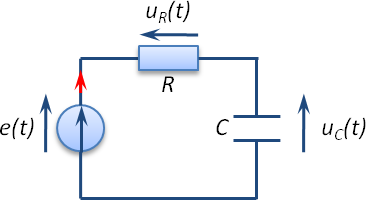
\includegraphics[width=.95\textwidth]{images/RC}
\end{center}
\end{minipage}

\subparagraph{}
\textit{Montrer que l'équation différentielle régissant la tension aux bornes du condensateur peut se mettre sous la forme :
$$
\dfrac{\text{d}u_C(t)}{\text{d}t} + \dfrac{u_C(t)}{\tau} = \dfrac{e(t)}{\tau}
$$
avec $\tau$ une constante à déterminer.}


Le circuit est commandé par un échelon de tension de la forme :
$$
\left\{
\begin{array}{l}
e(t) = E_0 \text{ si } $t>0$\\
0 \text{ sinon}
\end{array}
\right.
$$ 

\subparagraph{}
\textit{Déterminer, en justifiant votre réponse, la valeur de $u_c(0^+)$. }

\subparagraph{}
\textit{Montrer que la solution de l'équation différentielle régissant la charge du condensateur est de la forme :
$$
\forall t>0 \quad u_c(t) = E_0 \left( 1-e^{-\dfrac{t}{\tau}}\right)
$$
}

\begin{rem}
On prendra : 
\begin{itemize}
\item $R = 20\; k\Omega$;
\item $C=10 \;nF$.
\item $E=5\; V$;
\item temps de calcul : $T = 5\;ms$;
\item pas de calcul pour la solution théorique : $T/1000$;
\item pas de calcul pour la solution numérique : de $T/10$ à $T/1000$.
\end{itemize}
\end{rem}
\subparagraph{}
\textit{En utilisant Spyder, tracer la courbe correspondant à la charge du condensateur.}

\textbf{Connaissant la solution analytique de l'équation différentielle, on va maintenant chercher à tracer la solution numérique.}

\subparagraph{} 
\textit{En utilisant le schéma d'Euler explicite, déterminer la suite $u_n$ définie par récurrence pour tout $n\in \mathbb{N}$.}

\ifthenelse{\boolean{prof}}{
\begin{corrige}
On approxime $\dfrac{du_C(t)}{dt}\simeq \dfrac{u_C(t+h)-u_C(t)}{h}$

On pose $u_n=u_c(n\cdot h)$. On a alors 
$$
\dfrac{u_{n+1}-u_n}{h}  + \dfrac{u_n}{\tau} = \dfrac{e(t)}{\tau}
\Longleftrightarrow
u_{n+1}  = h\dfrac{e(t)}{\tau} - h\dfrac{u_n}{\tau} +u_n
= h\dfrac{e(t)}{\tau}  +u_n\left( 1-\dfrac{h}{\tau}\right)
$$
\end{corrige}
}{}

\subparagraph{}
\textit{On souhaite réaliser en Python la fonction \textsf{solveU} permettant de résoudre l'équation différentielle régissant la charge du condensateur. Quels paramètres la fonction doit-elle prendre comme argument ? Programmer la fonction.}

\subparagraph{}
\textit{Tracer sur un même graphe la solution analytique et la solution numérique pour des pas de résolution différents.}


Le circuit est maintenant commandé par un signal sinusoïdal de la forme :
$$
\left\{
\begin{array}{l}
e(t) = E_0 \sin \omega t \text{ si } $t>0$\\
0 \text{ sinon}
\end{array}
\right.
\quad
\text{ou}
\quad
\left\{
\begin{array}{l}
e(t) = E_0 \sin \left(2\pi f t\right) \text{ si } $t>0$\\
0 \text{ sinon}
\end{array}
\right.
$$ 



\subparagraph{}
\textit{Rechercher une solution numérique en tenant compte du nouveau signal d'entrée. Commenter l'allure de la courbe.}


\subparagraph{}
\textit{Réaliser un tracé pour $f = \{10;100;1\;000;10 \;000 \}$. Interpréter les résultats.}


\subparagraph{}
\textit{Que se passe-il quand le pas de calcul diminue. Que peut-on en conclure ? (Vous préciserez comment choisir le pas de calcul, en fonction de la constante de temps du circuit RC, pour avoir un bon compromis entre nombre d'itérations et validité (qualitative) de la solution numérique.)}


\subsection*{Exercice 2 -- Axe Emericc}
L'axe Emericc permet le déplacement de masses, grâce à un motoréducteur et un système pignon courroie.

\setcounter{subparagraph}{0}
\vspace{.25cm}

\begin{minipage}[c]{.4\linewidth}
\begin{center}
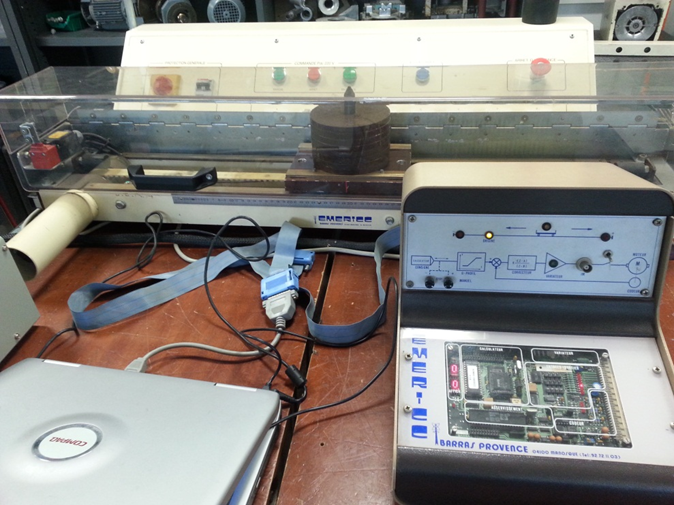
\includegraphics[width=.95\textwidth]{images/emericc}
\end{center}

\end{minipage} \hfill
\begin{minipage}[c]{.55\linewidth}
\begin{center}
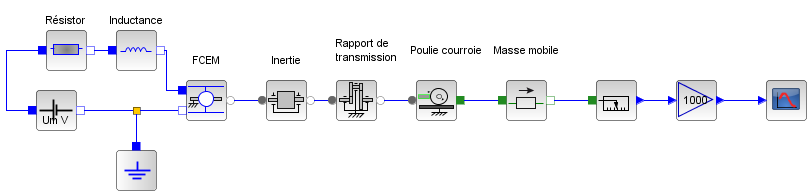
\includegraphics[width=\textwidth]{images/emericc_acausal}

\textit{Modélisation causale de l'axe Emericc en boucle ouverte}
\end{center}
\end{minipage}


\vspace{.25cm}

Dans le circuit électrique, l'expression de la loi des mailles se traduit par :
$$
u(t)= Ri(t)+L\dfrac{di(t)}{dt}+ e(t)
$$

Dans un moteur à courant continu, le couple est lié à l'intensité du courant et la fréquence de rotation est liée à la force contre électro motrice :
$$
C_m(t)=K_t i(t) \quad e(t)=K_e \omega_m(t)
$$

En isolant l'arbre moteur, le réducteur, le système poulie-courroie on peut calculer l'énergie cinétique de l'ensemble du système: 
$$
\mathcal{E}_c\left(E/\mathcal{R}\right)=\dfrac{1}{2}MV_{\text{chariot}/\mathcal{R}} ^2 + \dfrac{1}{2}J\omega_m^2
$$

D'après le théorème de l'énergie cinétique, en négligeant les frottements, on a :
$$
\dfrac{d\mathcal{E}_c\left(E/\mathcal{R}\right)}{dt}= C_m (t) \omega_m(t)
\Longleftrightarrow 
MV_{\text{chariot}/\mathcal{R}} \dot{V}_{\text{chariot}/\mathcal{R}} + 
J\dot{\omega}_m(t)\cdot\omega_m(t)= C_m (t) \omega_m(t)
$$

Par ailleurs, en utilisant le rapport de réduction ($k$) du réducteur et de la poulie courroie (diamètre $D$), on a $V_{\text{chariot}/\mathcal{R}}(t) = \omega_m(t)\cdot k \dfrac{D}{2} $. 

En conséquence, 
$$
M\omega_m(t)\cdot k \dfrac{D}{2} \dot{\omega}_m(t)\cdot k \dfrac{D}{2}  + 
J\dot{\omega}_m(t)\cdot\omega_m(t)= C_m (t) \omega_m(t)
\Longleftrightarrow 
M  \dfrac{D^2 k^2}{4} \dot{\omega}_m(t)  + 
J\dot{\omega}_m(t)= C_m (t)
$$

Au final, on peut donc écrire l'équation différentielle régissant le mouvement du chariot :
$$
u(t)= \dfrac{R}{K_t}C_m(t)+\dfrac{L}{K_t}\dot{C}_m(t)+ K_e\omega_m(t)
\Longleftrightarrow
u(t)= \dfrac{R}{K_t}\left( M  \dfrac{D^2 k^2}{4} \dot{\omega}_m(t)  + 
J\dot{\omega}_m(t)\right)+\dfrac{L}{K_t}\left( M  \dfrac{D^2 k^2}{4} \ddot{\omega}_m(t)  + 
J\ddot{\omega}_m(t)\right)+ K_e\omega_m(t)
$$

Soit :
\begin{equation} 
 \dfrac{R}{K_t}\left( M  \dfrac{D^2 k^2}{4}   + 
J\right)\dot{\omega}_m(t)+\dfrac{L}{K_t}\left( M  \dfrac{D^2 k^2}{4}  + 
J\right)\ddot{\omega}_m(t)+ K_e\omega_m(t)
=u(t)
\Longleftrightarrow
\alpha \omega_m(t) + \beta \dot{\omega}_m(t)+ \gamma \ddot{\omega}_m(t)  = u(t)
\end{equation}


\begin{rem}
Pour les applications numériques, on aura : 
\begin{itemize}
\item $M=10 \; kg$,
\item $D_p=0,0573\;m$;
\item $L=630\cdot 10^{-6} \; H$;
\item $R=4 \;\Omega$;
\item $k=66$;
\item $k_e=0,0342  \; SI$;
\item $k_t=0,0342 \; SI$;
\item $J_m=47\cdot 10^{-7} \; kg\cdot m^2$.
\end{itemize}
\end{rem}


\subparagraph{}
\textit{Préciser les unités des constantes $k_e$ et $k_t$.}

\subparagraph{}
\textit{Montrer que l'équation différentielle régissant la vitesse du chariot peut se mettre sous la forme :
$$
a V_{\left(\text{chariot}/\mathcal{R}\right)}
+ b \dot{V}_{\left(\text{chariot}/\mathcal{R}\right)}
+ c \ddot{V}_{\left(\text{chariot}/\mathcal{R}\right)}  = u(t)
$$
avec
$$c =    \dfrac{L}{K_t}\left( M  \dfrac{D^2 k^2}{4}  + J\right)\dfrac{2}{D_p k} 
\quad
b =  \dfrac{R}{K_t}\left( M  \dfrac{D^2 k^2}{4}   + J\right)\dfrac{2}{D_p k}   
\quad 
a= K_e\dfrac{2}{D_p k}$$
}

\ifthenelse{\boolean{prof}}{
\begin{corrige}
On a $V\left(\text{chariot}/\mathcal{R}\right) = k \omega_m(t) \dfrac{D_p}{2} $ 
$$
\alpha \omega_m(t) + \beta \dot{\omega}_m(t)+ \gamma \ddot{\omega}_m(t)  = u(t)
\Longrightarrow 
\dfrac{2}{D_p k} V\left(\text{chariot}/\mathcal{R}\right) = \omega_m(t) 
$$
\begin{equation} 
 \dfrac{R}{K_t}\left( M  \dfrac{D^2 k^2}{4}   + 
J\right)\dfrac{2}{D_p k} \dot{V}\left(\text{chariot}/\mathcal{R}\right)+\dfrac{L}{K_t}\left( M  \dfrac{D^2 k^2}{4}  + 
J\right)\dfrac{2}{D_p k} \ddot{V}\left(\text{chariot}/\mathcal{R}\right)+ K_e\dfrac{2}{D_p k} V\left(\text{chariot}/\mathcal{R}\right)
=u(t)
\end{equation}

On pose : 
\begin{itemize}
\item $c =    \dfrac{L}{K_t}\left( M  \dfrac{D^2 k^2}{4}  + 
J\right)\dfrac{2}{D_p k} $
\item $b =  \dfrac{R}{K_t}\left( M  \dfrac{D^2 k^2}{4}   + 
J\right)\dfrac{2}{D_p k}   $
\item $ a= K_e\dfrac{2}{D_p k}$
\end{itemize}
et 
$$
a V\left(\text{chariot}/\mathcal{R}\right)
+ b \dot{V}\left(\text{chariot}/\mathcal{R}\right)
+ c \ddot{V}\left(\text{chariot}/\mathcal{R}\right)  = u(t)
$$
\end{corrige}
}{}

\subparagraph{}
\textit{En utilisant le schéma d'Euler explicite, montrer que si on pose $v_1(t) =\dfrac{d{V}\left(\text{chariot}/\mathcal{R}\right)}{dt}$ et $v_2(t) ={V}\left(\text{chariot}/\mathcal{R}\right)$, 
résoudre l'équation différentielle, revient à calculer les termes des suites suivantes : 
$$
\left\{
\begin{array}{l}
v_2(n+1)= h \cdot v_1(t) + v_2(n)\\
v_1(n+1) =  h\dfrac{u(n) - a v_2(n)- b v_1(n)}{c} + v_1(n)
\end{array}
\right.
$$
On précisera les conditions initiales ($v_1(0)$ et $v_2(0)$).}

\ifthenelse{\boolean{prof}}{
\begin{corrige}
On a :
$$
a V\left(\text{chariot}/\mathcal{R}\right)
+ b \dot{V}\left(\text{chariot}/\mathcal{R}\right)
+ c \ddot{V}\left(\text{chariot}/\mathcal{R}\right)  = u(t)
\Longleftrightarrow 
\ddot{V}\left(\text{chariot}/\mathcal{R}\right) = \dfrac{u(t) - a V\left(\text{chariot}/\mathcal{R}\right)
- b \dot{V}\left(\text{chariot}/\mathcal{R}\right)}{c}
$$

Donc d'une part, 
$$
\left\{
\begin{array}{l}
\dfrac{dv_2(t)}{dt}= v_1(t)\\
\dfrac{dv_1(t)}{dt} = \ddot{V}\left(\text{chariot}/\mathcal{R}\right) = \dfrac{u(n) - a V\left(\text{chariot}/\mathcal{R}\right)
- b \dot{V}\left(\text{chariot}/\mathcal{R}\right)}{c}
\end{array}
\right.
\Longleftrightarrow
\left\{
\begin{array}{l}
\dfrac{dv_2(t)}{dt}= v_1(t)\\
\dfrac{dv_1(t)}{dt} =  \dfrac{u(t) - a v_2(n)- b v_1(n)}{c}
\end{array}
\right.
$$

D'autre part, 
$$
\left\{
\begin{array}{l}
\dfrac{dv_1(t)}{dt}\simeq \dfrac{v_1(n+1)-v_1(n)}{h}\\
\dfrac{dv_2(t)}{dt} \simeq \dfrac{v_2(n+1)-v_2(n)}{h}
\end{array}
\right.
$$

On a donc :
$$
\left\{
\begin{array}{l}
 \dfrac{v_2(n+1)-v_2(n)}{h}= v_1(n)\\
\dfrac{v_1(n+1)-v_1(n)}{h} =  \dfrac{u(n) - a v_2(n)- b v_1(n)}{c}
\end{array}
\right.
\Longleftrightarrow
\left\{
\begin{array}{l}
v_2(n+1)= h \cdot v_1(t) + v_2(n)\\
v_1(n+1) =  h\dfrac{u(t) - a v_2(n)- b v_1(n)}{c} + v_1(n)
\end{array}
\right.
$$

\begin{rem}
On peut noter que :
$$
\left[
\begin{array}{c}
 \dot{V}_c \\
 \ddot{V}_c
\end{array}
\right]
= 
\left[\begin{array}{cc}
 0 & 1 \\
-\dfrac{a}{c} & -\dfrac{b}{c}
\end{array}
\right]
\cdot
\left[
\begin{array}{c}
 {V}_c \\
 \dot{V}_c
\end{array}
\right]
+
\left[
\begin{array}{c}
 0 \\
 \dfrac{u(t)}{c}
\end{array}
\right]
$$
\end{rem}
\end{corrige}
}{}


\subparagraph{}
\textit{Pour un échelon de tension de $21,3\;V$, réaliser une fonction permettant de calculer le nième terme des suites $v_1$ et $v_2$.}
\ifthenelse{\boolean{prof}}{
\begin{corrige}
\end{corrige}
}{}



\subparagraph{}
\textit{Tracer la courbe de correspondant à la vitesse du chariot pour un temps de simulation de 0,3 secondes. Pour quelle valeur du pas de calcul, la solution commence-t-elle à diverger.}


\subparagraph{}
\textit{Tracer l'allure de la courbe de position du chariot. Commenter son allure. }

\vspace{.25cm}

La bilbiothèque Scipy de Python permet de résoudre les équations différentielles. Pour résoudre l'équation précédente, la méthode est la suivante :
\begin{py}
\begin{python}
from scipy.integrate import odeint

def emeric(v_dv_ddv,t):
    v,dv = v_dv_ddv
    return [dv,(21.3-a*v-b*dv)/(c)]

t=linspace(0,0.3,1000)
sol = odeint(emeric, (0, 0), t)
plot(sol)
\end{python}
\end{py}
\subparagraph{}
\textit{En utilisant la documentation que vous trouverez sur internet, expliquer le morceau de programme ci-dessus. Saisir le code et exécuter le fichier. Quel est le résultat obtenu ? Python affiche deux courbes, quelles sont-elles ? Les résultats vous semblent-ils comparables avec votre programme initial ?}


\end{document}

